\documentclass[totpages,helvetica,openbib,italian]{europecv}
\usepackage[T1]{fontenc}
\usepackage{graphicx}
\usepackage[a4paper,top=1.27cm,left=1cm,right=1cm,bottom=2cm]{geometry}
\usepackage[italian]{babel}
\usepackage{bibentry}
\usepackage{url}

%\renewcommand{\ttdefault}{phv} % Uses Helvetica instead of fixed width font
\renewcommand{\normalsize}{\fontsize{10}{0}\selectfont}

\ecvname{Diego Russo}
\ecvaddress{Via G. Garibaldi 40, 05021, Acquasparta (TR), Italia}
\ecvtelephone[+39 334 5873886]{+39 0744 930614}
\ecvemail{\url{diegor.it@gmail.com} - Personale, gtalk, MSN \\& \url{diego.russo@forinicom.it} - Forinicom S.r.l.}
\ecvhomepage{\url{http://www.diegor.it}}
\ecvnationality{Italiana}
\ecvdateofbirth{30 aprile 1983}
\ecvgender{Maschio}
\ecvbeforepicture{\raggedleft}
\ecvpicture[width=3cm]{diegor.jpg}
\ecvafterpicture{\ecvspace{-3cm}} 
\ecvfootnote{Per ulteriori informazioni: \url{http://europass.cedefop.eu.int}\\
\textcopyright~European Communities, 2003.}

\begin{document}
    \begin{center}
        \hspace{1pt}
        \vspace{2cm}
    
        {\scshape \textbf{\Huge Diego Russo}}
    
        \vspace{1cm}
    
        {\scshape \textbf{\large \underline{Curriculum Vitae}}}
    
        \vspace{0.25cm}
    
        aggiornato al \emph{\textbf{10 marzo 2010}}
        
        \vspace{2cm}
        
        \begin{figure}[htbp] 
            \begin{center} 
                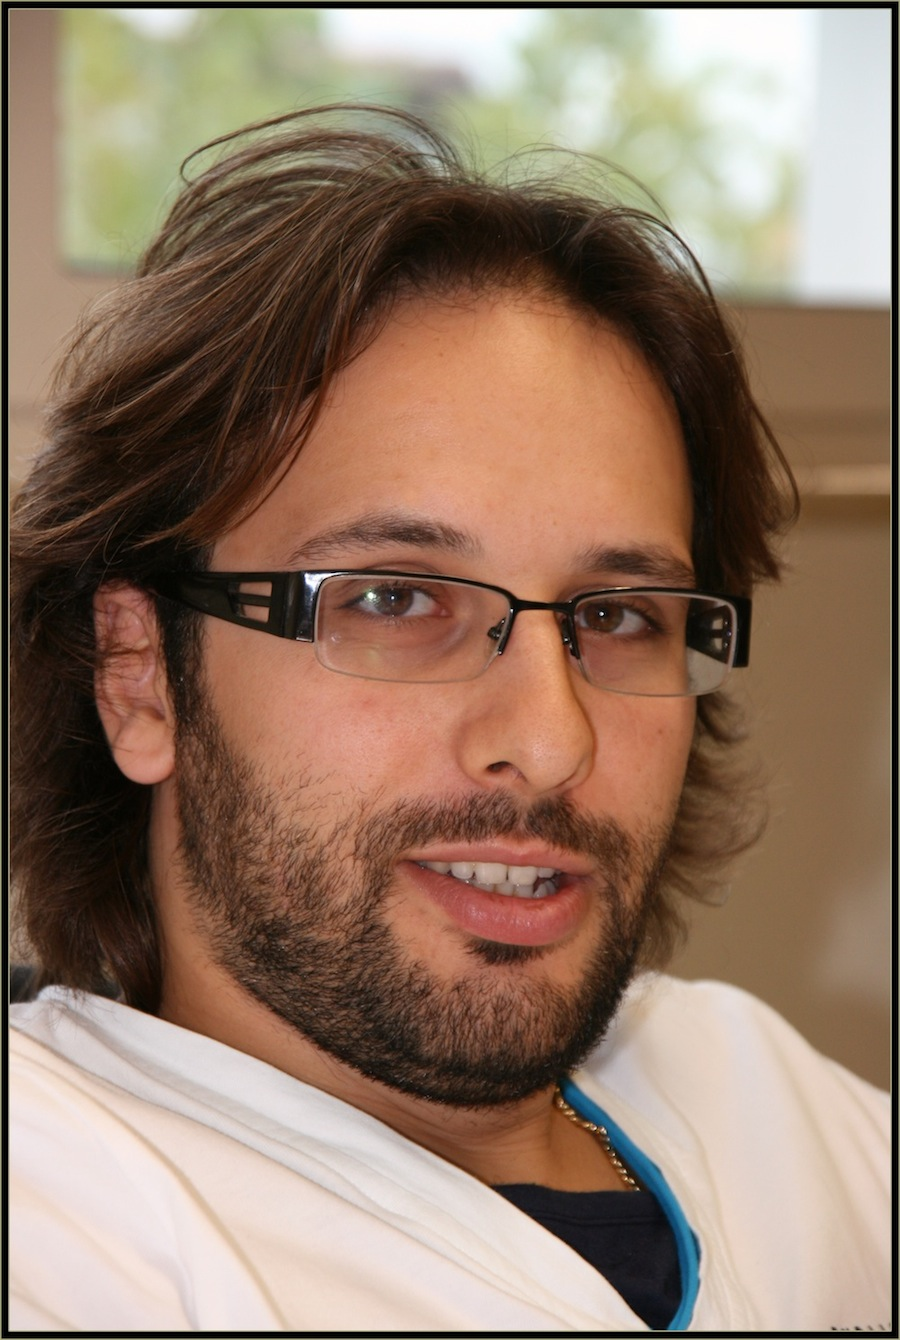
\includegraphics[width=10cm]{io.jpg}
            \end{center} 
        \end{figure}
        
    \end{center}
\pagebreak
\selectlanguage{italian}

\begin{europecv}
\ecvpersonalinfo[5pt]

%\ecvitem{\large\textbf{Impiego ricercato/ Settore di competenza}}{\large\textbf{Programmatore Python, Django.}}

\ecvsection{Esperienza professionale}

\ecvitem{Date}{\textbf{Dal 26 aprile 2008 ad Oggi}}
\ecvitem{Lavoro o posizione ricoperti}{Programmatore, sistemista (lavoratore con contratto di apprendistato part-time, 25 ore)}
\ecvitem{Principali attivit\'a e responsabilit\`a}{Sviluppo di un progetto che mira ad offrire connettivit\'a e servizi integrati (videosorveglianza, voip) alle pubbliche amministrazioni, aziende e privati. Punti previsti dal contratto:
\begin{itemize}
    \item conoscere i prodotti ed i servizi del settore e del contesto aziendale: reti Mesh e gararchiche, servizi VoIP e videosorveglianza, sicurezza delle reti wired e wireless;
    \item conoscere e saper applicare le basi tecniche e scientifiche della professionalit\'a;
    \item conoscere e saper utilizzare tecniche e metodi di lavoro con particolare riferimento allo sviluppo software e alla documentazione del codice;
    \item conoscere e saper utilizzare strumenti e tecnologie di lavoro (attrezzature, macchinari e strumenti di lavoro), in particolare ambiente di sviluppo Linux, piattaforma di sviluppo Linux/OSX, linguaggi di programmazione Python e database PostgresSQL/MySQL;
    \item conoscere ed utilizzare misure di sicurezza individuale e per la tutela ambientale;
    \item conoscere le innovazioni di prodotto, di processo, di contesto e di settore.
\end{itemize}
Inoltre ho sviluppato applicazioni in python e in python-django sia per il lavoro quotidiano del reparto tecnico e non sia di pura ricerca e sviluppo. A tal senso ho implementato da zero un server per gestire il \textbf{servizio di hotspot}.}
\ecvitem{Nome e indirizzo del datore di lavoro}{Forinicom srl, Via del Popolo, 9 Bastia Umbra, 06083, 0758001868, \url{http://www.forinicom.it}}
\ecvitem{Tipo di attivit\`a o settore}{Settore telecomunicazioni}

\ecvitem{}{}

\ecvitem{Date}{\textbf{Dal 03 settembre 2009 ad Oggi}}
\ecvitem{Lavoro o posizione ricoperti}{Programmatore (lavoratore con contratto a progetto, part-time)}
\ecvitem{Principali attivit\'a e responsabilit\`a}{Sviluppo di un'applicazione gestionale per il comune di Bettona in django, python, postgresql, linux, apache, per l'informatizzazione dei servizi per la gestione delle anagrafiche nonch\'e delle pratiche edilizie ed urbanistiche e del calcolo della tassa ICI con aggiornamenti dei dati catastali. Utilizzo di un server per il controllo di versione (GIT). Inoltre in questa fase c'\'e stata il completamento del prodotto con la relativa commercializzazione.}
\ecvitem{Nome e indirizzo del datore di lavoro}{Consorzio Miles - Servizi Integrati, CF 04881101002, Via Rocca di Papa 21, Roma}
\ecvitem{Tipo di attivit\`a o settore}{Servizi integrati per la pubblica amministrazione}

\ecvitem{}{}

\ecvitem{Date}{\textbf{Dal 01 agosto 2007 al 31 agosto 2008}}
\ecvitem{Lavoro o posizione ricoperti}{Programmatore (lavoratore con contratto a progetto, full-time)}
\ecvitem{Principali attivit\'a e responsabilit\`a}{Sviluppo di un'applicazione gestionale per il comune di Bettona in django, python, postgresql, linux, apache, per l'informatizzazione dei servizi per la gestione delle anagrafiche nonch\'e delle pratiche edilizie ed urbanistiche e del calcolo della tassa ICI con aggiornamenti dei dati catastali. Utilizzo di un server per il controllo di versione (SVN), con relativa interfaccia web (trac) per la gestione dei ticket.}
\ecvitem{Nome e indirizzo del datore di lavoro}{Consorzio Miles - Servizi Integrati, CF 04881101002, Via Rocca di Papa 21, Roma}
\ecvitem{Tipo di attivit\`a o settore}{Servizi integrati per la pubblica amministrazione}

\ecvitem{}{}

\ecvitem{Date}{\textbf{Dal 11 dicembre 2006 al 30 luglio 2007}}
\ecvitem{Lavoro o posizione ricoperti}{Programmatore (lavoratore con contratto a progetto, full-time)}
\ecvitem{Principali attivit\'a e responsabilit\`a}{Sviluppo di un'applicazione gestionale per il comune di Bettona in django, python, postgresql, linux, apache, per l'informatizzazione dei servizi per la gestione delle anagrafiche nonch\'e delle pratiche edilizie ed urbanistiche e del calcolo della tassa ICI con aggiornamenti dei dati catastali. Utilizzo di un server per il controllo di versione (SVN), con relativa interfaccia web (trac) per la gestione dei ticket.}
\ecvitem{Nome e indirizzo del datore di lavoro}{Consorzio Miles - Servizi Integrati, CF 04881101002, Via Rocca di Papa 21, Roma}
\ecvitem{Tipo di attivit\`a o settore}{Servizi integrati per la pubblica amministrazione}

\ecvitem{}{}

\ecvitem{Date}{\textbf{Dal 30 luglio 2006 al 30 dicembre 2006}}
\ecvitem{Lavoro o posizione ricoperti}{Tesista (Wireless Broadband Network)}
\ecvitem{Principali attivit\'a e responsabilit\`a}{Wireless Broadband Network - progetto \textbf{WeConnect} - Banda larga su reti wireless:
    \begin{itemize}
        \item Ampia conoscenza della rete wireless e del suo funzionamento
        \item Buona conoscenza della normativa che regola il Wi-Fi
        \item Ottima conoscenza del sistema RouterOS (www.mikrotik.com)
        \item Conoscenza del protocollo AAA e del server FreeRADIUS
        \item Amministrazione dei vari servizi di rete: mail (postfix), server web (apache), DNS (pdns), firewall (iptables), database (postgresql), hotspot (chillispot), OS Debian, Voyage (OS per sistemi embedded, basata su Debian)
    \end{itemize} 
}
\ecvitem{Nome e indirizzo del datore di lavoro}{WEDOIT s.a.s. - Via Protomartiri Francescani,26 - 06088 Assisi (PG)}
\ecvitem{Tipo di attivit\`a o settore}{Soluzioni informatiche}

\ecvitem{}{}

\ecvitem{Date}{\textbf{Dal 14 novembre 2005 al 30 maggio 2006}}
\ecvitem{Lavoro o posizione ricoperti}{Stagista (S.E.O. Search Engine Optimization)}
\ecvitem{Principali attivit\'a e responsabilit\`a}{
    \begin{itemize}
        \item Conoscenza del SEO e dei sui meccanismi. Ottimizzazione di un sito per il S.E.O.
        \item Tecniche di Pageranking e link popularity
        \item Sistemista di un server virtuale, basato su Debian
        \item Apprendimento del linguaggio di programmazione Python
    \end{itemize}
}
\ecvitem{Nome e indirizzo del datore di lavoro}{WEDOIT s.a.s. - Via Protomartiri Francescani,26 - 06088 Assisi (PG)}
\ecvitem{Tipo di attivit\`a o settore}{Soluzioni informatiche}

\ecvitem{}{}

\ecvitem{Date}{\textbf{Marzo 2002}}
\ecvitem{Lavoro o posizione ricoperti}{Stagista (Stage abbinato al progetto IFS, Impresa Formativa Simulata)}
\ecvitem{Principali attivit\'a e responsabilit\`a}{Gestione della rete interna dell'impresa}
\ecvitem{Nome e indirizzo del datore di lavoro}{IOSA CARLO S.r.l. - 05100 TERNI - Via Pallotta n. 7 - Tel. (0744) 2460 - Fax (0744) 246035 - P.IVA 00072550551 - \url{http://www.iosacarlo.com} - \url{iosacarlo@iosacarlo.com}}
\ecvitem{Tipo di attivit\`a o settore}{Impresa smaltimento rifiuti}

\ecvitem{}{}

\ecvsection{Istruzione e formazione}

\ecvitem{Date}{\textbf{Da Ottobre 2008 a oggi}}
\ecvitem{Titolo della qualifica rilasciata}{Iscritto alla specializzazione di Informatica, indirizzo di ``Sicurezza Informatica''}
\ecvitem{Principali tematiche/competenze professionali possedute}{Sostenuti i seguenti esami con relativa votazione:\begin{itemize}
    \item Simulazione: 30 e lode
    \item Programmazione Avanzata: 30 e lode
    \item Sistemi operativi avanzati: 30 e lode
    \item Laboratorio di Sistemi operativi avanzati: 30 e lode
\end{itemize}}
\ecvitem{Nome e tipo d\'organizzazione erogatrice dell\'istruzione e formazione}{Universit\'a degli studi di Perugia, Dipartimento di Informatica}
\ecvitem{Livello nella classificazione nazionale o internazionale}{-}

\ecvitem{}{}

\ecvitem{Date}{\textbf{Dal 17 Febbraio 2010 ad Oggi}}
\ecvitem{Titolo della qualifica rilasciata}{Iscritto al 4$^\circ$ modulo di Lingua spagnola}
\ecvitem{Principali tematiche/competenze professionali possedute}{-}
\ecvitem{Nome e tipo d'organizzazione erogatrice dell'istruzione e formazione}{Istituto comprensivo ``Volumnio'' Ponte San Giovanni - Perugia}
\ecvitem{Livello nella classificazione nazionale o internazionale}{-}

\ecvitem{}{}

\ecvitem{Date}{\textbf{Dal 14 Ottobre 2009 al 12 Febbraio 2010}}
\ecvitem{Titolo della qualifica rilasciata}{Attestato di frequenza di 42 ore su 50 del 3$^\circ$ modulo di Lingua spagnola}
\ecvitem{Principali tematiche/competenze professionali possedute}{\begin{itemize}
    \item comprendere frasi ed espressioni di uso frequente relativi ad ambiti di mmediata rilevanza
    \item saper descrivere in termini semplici aspetti della propria storia e delle proprie esperienze
    \item saper parlare dell'ambiente circostante e saper esprimere bisogni, intenzioni e previsioni
\end{itemize}}
\ecvitem{Nome e tipo d'organizzazione erogatrice dell'istruzione e formazione}{Istituto comprensivo ``Volumnio'' Ponte San Giovanni - Perugia}
\ecvitem{Livello nella classificazione nazionale o internazionale}{-}

\ecvitem{}{}

\ecvitem{Date}{\textbf{Da febbraio 2007 a luglio 2007}}
\ecvitem{Titolo della qualifica rilasciata}{Patente di operatore di stazione di radioamatore di classe A}
\ecvitem{Principali tematiche/competenze professionali possedute}{Corso per aspiranti radioamatori:
\begin{itemize}
    \item Ottima conoscenza delle basi della radiotecnica
    \item Ottima conoscenza delle apparecchiature radio e del loro funzionamento
    \item Conoscenza delle basi della fisica e chimica (magnetismo,  elettromagnetismo)
\end{itemize}}
\ecvitem{Nome e tipo d'organizzazione erogatrice dell'istruzione e formazione}{C.I.S.A.R. Sezione di Foligno}
\ecvitem{Livello nella classificazione nazionale o internazionale}{IDONEO, Nominativo internazionale \textbf{IZ0OVB}}

\ecvitem{}{}

\ecvitem{Date}{\textbf{Dal 10 aprile 2007 ad Oggi}}
\ecvitem{Titolo della qualifica rilasciata}{-}
\ecvitem{Principali tematiche/competenze professionali possedute}{Formazione personale in Second Life:
\begin{itemize}
    \item Builder di edifici e costruzioni
    \item Scripting in LSL (Linden Scripting Language) e tecniche per la costruzione in SL.
    \item Conoscenza dei trucchi e dei bugs del metaverso
    \item Creazione di molti edifici in varie isole di SL: Milano, Marostica, Assisi
\end{itemize}}
\ecvitem{Nome e tipo d'organizzazione erogatrice dell'istruzione e formazione}{Formazione personale}
\ecvitem{Livello nella classificazione nazionale o internazionale}{Ottimo apprendimento del metaverso e dei meccanismi che lo animano}

\ecvitem{}{}

\ecvitem{Date}{\textbf{Da Marzo 2007 a Luglio 2007}}
\ecvitem{Titolo della qualifica rilasciata}{-}
\ecvitem{Principali tematiche/competenze professionali possedute}{Formazione personale su piattaforma Plone-Zope:
\begin{itemize}
    \item Sistemista di server virtuali ospitanti siti in plone.
    \item Programmatore in python di script per il controllo di gestione
\end{itemize}}
\ecvitem{Nome e tipo d'organizzazione erogatrice dell'istruzione e formazione}{Formazione personale}
\ecvitem{Livello nella classificazione nazionale o internazionale}{Conoscenza del CMS Plone e maggiore padronanza del linguaggio Python}

\ecvitem{}{}

\ecvitem{Date}{\textbf{Dal 22 febbraio 2007 al 12 marzo 2007}}
\ecvitem{Titolo della qualifica rilasciata}{}
\ecvitem{Principali tematiche/competenze professionali possedute}{Formazione personale in programmazione PHP e Postgresql:
\begin{itemize}
    \item Sviluppo di una piccola applicazione in PHP e postgresql per la gestione delle anagrafiche di clienti.
\end{itemize}}
\ecvitem{Nome e tipo d'organizzazione erogatrice dell'istruzione e formazione}{Formazione personale}
\ecvitem{Livello nella classificazione nazionale o internazionale}{Maggiore conoscenza del PHP}

\ecvitem{}{}

\ecvitem{Date}{\textbf{Dal 19 marzo 2007 al 23 marzo 2007}}
\ecvitem{Titolo della qualifica rilasciata}{Attestato di partecipazione al corso}
\ecvitem{Principali tematiche/competenze professionali possedute}{\begin{itemize}
    \item Grammatica di base della lingua spagnola
    \item Cultura generale spagnola
\end{itemize}}
\ecvitem{Nome e tipo d'organizzazione erogatrice dell'istruzione e formazione}{Inhispania Intlance S.L / CIF:B83744847 , Montera 10-12, 1-1. 28013, Madrid (Spain)}
\ecvitem{Livello nella classificazione nazionale o internazionale}{Valutazioni\footnote{Valutazione in accordo con il ``Common European Framework of Reference for Languages''}:\begin{itemize}
    \item Espressione orale: A2
    \item Espressione scritta: A2
    \item Comprensione orale: A2
    \item Comprensione scritta: A2
    \item Interazione orale: A2
\end{itemize}}

\ecvitem{}{}

\ecvitem{Date}{\textbf{03-10-25 Marzo 2007}}
\ecvitem{Titolo della qualifica rilasciata}{Attestato di partecipazione al corso}
\ecvitem{Principali tematiche/competenze professionali possedute}{\begin{itemize}
    \item .NET Framework Architeture (2.0)
    \item ADO.NET
    \item ASP.NET (web forms, Page, controlli, sicurezza)
    \item C\#
    \item Web Service
    \item Ajax.net
    \item Microsoft Visual Studio 2005
\end{itemize}}
\ecvitem{Nome e tipo d'organizzazione erogatrice dell'istruzione e formazione}{O.S.MO.S.IT, Via Strozzacapponi, 85, 06071 Castel del Piano (Pg)}
\ecvitem{Livello nella classificazione nazionale o internazionale}{Conoscenza di base della programmazione Microsoft}

\ecvitem{}{}

\ecvitem{Date}{\textbf{Da novembre 2007 ad OGGI}}
\ecvitem{Titolo della qualifica rilasciata}{}
\ecvitem{Principali tematiche/competenze professionali possedute}{Ottime conoscenze del sistema operativo OSX 10.5 (Leopard) ed OSX 10.6 (Snow Leopard):
\begin{itemize}
    \item Amministrazione di un sistema OSX 10.5 (Leopard)
    \item Buona conoscenza del sottosistema BSD
    \item Ottima conoscenza del prodotto
\end{itemize}}
\ecvitem{Nome e tipo d'organizzazione erogatrice dell'istruzione e formazione}{Formazione personale}
\ecvitem{Livello nella classificazione nazionale o internazionale}{Ottima padronanza del sistema operativo OSX}

\ecvitem{}{}

\ecvitem{Date}{\textbf{Da settembre 2006 a febbraio 2007}}
\ecvitem{Titolo della qualifica rilasciata}{Pubblicazione del libro UbuntuSemplice con conseguente donazione a Canonical Ltd.}
\ecvitem{Principali tematiche/competenze professionali possedute}{\begin{itemize}
    \item Contributor, autore di molti capitoli e sistemista del sistema informatico per \url{http://www.ubuntusemplice.org/}
    \item Amministrazione di un server virtuale Debian
    \item Configurazione ed utilizzo del software collaborativo MediaWiki per la stesura e composizione del libro.
    \item Configurazione del server web apache
    \item Configurazione di una mailing list per la gestione dei capitoli del libro con gli altri contributor
\end{itemize}}
\ecvitem{Nome e tipo d'organizzazione erogatrice dell'istruzione e formazione}{Progetto Ubuntusemplice - \url{http://www.ubuntusemplice.org/)}}
\ecvitem{Livello nella classificazione nazionale o internazionale}{Ottima conoscenza del sistema operativo Ubuntu}

\ecvitem{}{}

\ecvitem{Date}{\textbf{01-02-03 Dicembre 2006}}
\ecvitem{Titolo della qualifica rilasciata}{Attestato di partecipazione al corso}
\ecvitem{Principali tematiche/competenze professionali possedute}{Corso di formazione sulla sicurezza e certificazioni ISO:
\begin{itemize}
    \item ISO 27001:2005
    \item Politica per la sicurezza delle informazioni
    \item Analisi dei rischi (RA)
    \item Analisi dei controlli della ISO 17799:2005
    \item Trattamento dei rischi (RTP)
    \item Processo di certificazione
    \item Panorama delle certificazioni esistenti per gli audit
    \item Piano di audit e checklist
    \item Rapporto di audit
    \item Uno sguardo alle future certificazioni
\end{itemize}}
\ecvitem{Nome e tipo d'organizzazione erogatrice dell'istruzione e formazione}{WEDOIT s.a.s. - Via Protomartiri Francescani, 26 - 06088 Assisi (PG)}
\ecvitem{Livello nella classificazione nazionale o internazionale}{Conoscenza dei processi di certificazione ISO}

\ecvitem{}{}

\ecvitem{Date}{\textbf{Da ottobre 2002 a Novembre 2006}}
\ecvitem{Titolo della qualifica rilasciata}{\textbf{Laurea triennale (nuovo ordinamento)}}
\ecvitem{Principali tematiche/competenze professionali possedute}{Laurea triennale in informatica, indirizzo ``Reti di computer'':
\begin{itemize}
    \item Matematica (analitica e discreta)
    \item Programmazione (C, Java, Php, html, xml, xsl, dtd, Pascal, scripting bash e csh, VB.NET, VRML)
    \item DataBase (Mysql, MS Access e loro interazioni con liguaggi di
    \item programmazione)
    \item Reti (ATM, xDSL, Mpls, X.25, Frame Relay), tipologie (wireless, wired) e loro interazione
    \item Conoscenza di sistemi multimediali
    \item Cenni di calcolo parallelo (mpi)
\end{itemize}}
\ecvitem{Nome e tipo d'organizzazione erogatrice dell'istruzione e formazione}{Universit\'a degli studi di Perugia, Dipartimento di Informatica}
\ecvitem{Livello nella classificazione nazionale o internazionale}{\textbf{102/110}}

\ecvitem{}{}

\ecvitem{Date}{\textbf{Da ottobre 2005 a Maggio 2006}}
\ecvitem{Titolo della qualifica rilasciata}{-}
\ecvitem{Principali tematiche/competenze professionali possedute}{\begin{itemize}
    \item Studio del linguaggio di programmazione Python, con l'implementazione di alcune applicazione orientate al S.E.O.
    \item Studio del linguaggio di programmazione PHP, per lo sviluppo di alcune applicazioni orientate al S.E.O.
\end{itemize}}
\ecvitem{Nome e tipo d'organizzazione erogatrice dell'istruzione e formazione}{Auto formazione}
\ecvitem{Livello nella classificazione nazionale o internazionale}{}

\ecvitem{}{}

\ecvitem{Date}{\textbf{Da settembre 1996 a giugno 2002}}
\ecvitem{Titolo della qualifica rilasciata}{\textbf{Diploma in ragioniere programmatore (progetto Mercurio)}}
\ecvitem{Principali tematiche/competenze professionali possedute}{Materie previste dal percorso di studio dell'Istituto Tecnico Commerciale, definito dal Ministero dell'Istruzione, ovvero:
\begin{itemize}
    \item Scienze della Materia
    \item Matematica e Laboratorio
    \item Scienze della Natura
    \item Trattamento Testi e Dati
    \item Seconda lingua straniera (Francese)
    \item Diritto ed Economia
    \item Economia Aziendale
    \item Economia Politica e Scienza delle Finanze
    \item Lingua e letteratura italiana
    \item Storia
    \item Informatica Gestionale
    \item Matematica applicata
    \item Prima lingua straniera (Inglese)
    \item Diritto
\end{itemize}}
\ecvitem{Nome e tipo d'organizzazione erogatrice dell'istruzione e formazione}{Ministero della Pubblica Istruzione - I.T.C. ``Federico Cesi'', Terni}
\ecvitem{Livello nella classificazione nazionale o internazionale}{\textbf{85/100}}

\ecvitem{}{}

\ecvitem{Date}{\textbf{Dal 2001 al 2002}}
\ecvitem{Titolo della qualifica rilasciata}{Attestato di frequenza}
\ecvitem{Principali tematiche/competenze professionali possedute}{Progetto Nazionale IFS (\textbf{Impresa Formativa Simulata}). Simulazione di un'impresa di smaltimento rifiuti, affiancati dall'impresa Iosa Carlo S.r.l. (\url{http://www.iosacarlo.com}). Nell'ambito del progetto ho coordinato il lavoro di tutti gli studenti, realizzando l'organigramma dell'azienda simulata e programmando il sito dell'azienda.}
\ecvitem{Nome e tipo d'organizzazione erogatrice dell'istruzione e formazione}{Ministero della Pubblica Istruzione - I.T.C. ``Federico Cesi'', Terni}
\ecvitem{Livello nella classificazione nazionale o internazionale}{-}

\ecvitem{}{}

\ecvitem{Date}{\textbf{Dal 24 settembre 2001 al 14 ottobre 2001}}
\ecvitem{Titolo della qualifica rilasciata}{Attestato di frequenza}
\ecvitem{Principali tematiche/competenze professionali possedute}{Svoltasi l'attivit\'a di tutor/referente di un gruppo di altri 6 studenti/tutor, per le attivit\'a di POTENZIAMENTO DI ITALIANO delle prime classi, in ambito del progetto ``Accoglienza, Recupero, Potenziamento nelle Prime Classi''. L'attivit\'a \'e consistita nell'affiancare i Docenti di Lettere al fine di offrire un valido supporto agli alunni delle Prime Classi nell'utilizzo del Computer, per poter eseguire attivit\'a di approfondimento con il mezzo multimediale, attraverso esercitazioni con un CD-Rom di Grammatica. \textbf{Ottenute ottime capacit\'a relazionali, organizzative ed ottime competenze nell'insegnamento di materie tecniche.}}
\ecvitem{Nome e tipo d'organizzazione erogatrice dell'istruzione e formazione}{Ministero della Pubblica Istruzione - I.T.C. ``Federico Cesi'', Terni}
\ecvitem{Livello nella classificazione nazionale o internazionale}{-}

\ecvitem{}{}

\ecvitem{Date}{\textbf{Dal 7 dicembre 2001 al 09 dicembre 2001}}
\ecvitem{Titolo della qualifica rilasciata}{Attestato di frequenza}
\ecvitem{Principali tematiche/competenze professionali possedute}{Partecipazione all'organizzazione del ``Pluto Meeting 2001'', tenuto presso il suddetto istituto.}
\ecvitem{Nome e tipo d'organizzazione erogatrice dell'istruzione e formazione}{Ministero della Pubblica Istruzione - I.T.C. ``Federico Cesi'', Terni}
\ecvitem{Livello nella classificazione nazionale o internazionale}{-}

\ecvitem{}{}

\ecvitem{Date}{\textbf{Dal 26 marzo 2001 al 02 aprile 2001}}
\ecvitem{Titolo della qualifica rilasciata}{Attestato di frequenza}
\ecvitem{Principali tematiche/competenze professionali possedute}{Partecipazione alla ``XI Settimana della cultura scientifica e tecnologica'', realizzando sia la locandina che il programma provinciale della settimana delle scienze in Adobe Photoshop 5.5 ed in Corel Draw 8.0, impegnandosi sia in orario curriculare che extra-curriculare pomeridiano con grande devozione, senso della responsabilit\'a, fungendo anche da punto di riferimento per tutti gli studenti del biennio che hanno partecipato al progetto.}
\ecvitem{Nome e tipo d'organizzazione erogatrice dell'istruzione e formazione}{Ministero della Pubblica Istruzione - I.T.C. ``Federico Cesi'', Terni}
\ecvitem{Livello nella classificazione nazionale o internazionale}{-}

\ecvitem{}{}

\ecvitem{Date}{\textbf{Anno 2001}}
\ecvitem{Titolo della qualifica rilasciata}{Attestato di frequenza}
\ecvitem{Principali tematiche/competenze professionali possedute}{Corso di alfabetizzazione di base in funzione di tutor di 40 ore complessive ad un gruppo di 30 persone, con et\'a superiore al 65 anni. Ho svolto inoltre il ruolo di coordinatore del progetto stilando il programma e coordinando i miei aiutanti.}
\ecvitem{Nome e tipo d'organizzazione erogatrice dell'istruzione e formazione}{Ministero della Pubblica Istruzione - I.T.C. ``Federico Cesi'', Terni}
\ecvitem{Livello nella classificazione nazionale o internazionale}{-}

\ecvitem{}{}

\ecvitem{Date}{\textbf{Anno 2001}}
\ecvitem{Titolo della qualifica rilasciata}{Attestato di frequenza}
\ecvitem{Principali tematiche/competenze professionali possedute}{Corso di informatica di base in funzione di tutor (progetto 20 Studenti) di 30 ore complessive su applicazioni office (Word, Excel) ed Internet}
\ecvitem{Nome e tipo d'organizzazione erogatrice dell'istruzione e formazione}{Ministero della Pubblica Istruzione - I.T.C. ``Federico Cesi'', Terni}
\ecvitem{Livello nella classificazione nazionale o internazionale}{-}

\ecvitem{}{}

\ecvitem{Date}{\textbf{16-17-18 novembre 2000}}
\ecvitem{Titolo della qualifica rilasciata}{Attestato di frequenza}
\ecvitem{Principali tematiche/competenze professionali possedute}{Exposcuola - Salone del confronto tra le proposte formative dell'Europa e del Mediterraneo - Paestum hotel Arison}
\ecvitem{Nome e tipo d'organizzazione erogatrice dell'istruzione e formazione}{Ministero della Pubblica Istruzione - I.T.C. ``Federico Cesi'', Terni}
\ecvitem{Livello nella classificazione nazionale o internazionale}{-}

\ecvitem{}{}

\ecvitem{Date}{\textbf{Da Giugno 2001 a OGGI}}
\ecvitem{Titolo della qualifica rilasciata}{}
\ecvitem{Principali tematiche/competenze professionali possedute}{\begin{itemize}
    \item Installazione, amministrazione, configurazione di una Debian 3.0-4.0-5.0 e derivate
    \item Configurazione del kernel
    \item Compilazione del kernel
    \item Scripting bash
    \item Configurazione dei servizi di rete (apache, ftp, irc, mail)
    \item Conoscenza ottimale del sistema
    \item Conoscenza ottimale del gestore dei pacchetti (deb)
\end{itemize}}
\ecvitem{Nome e tipo d'organizzazione erogatrice dell'istruzione e formazione}{Auto formazione}
\ecvitem{Livello nella classificazione nazionale o internazionale}{Ottime conoscenze in ambito open source, linux, Debian e derivate}

\ecvitem{}{}

\ecvitem{Date}{\textbf{Da Settembre 2000 a Giugno 2001}}
\ecvitem{Titolo della qualifica rilasciata}{}
\ecvitem{Principali tematiche/competenze professionali possedute}{
\begin{itemize}
    \item Installazione, amministrazione, configurazione di una Slackware 7.1
    \item Configurazione del kernel
    \item Compilazione del kernel
    \item Compilazione a mano di tutto il sistema con l'ausilio di script bash da me create
    \item Configurazione dei servizi di rete (apache, ftp, irc, mail)
    \item Scrittura di patch personalizzate
    \item Studio del del linguaggio C
    \item Studio del libro ``Appunti di informatica libera''
\end{itemize}}
\ecvitem{Nome e tipo d'organizzazione erogatrice dell'istruzione e formazione}{Auto formazione}
\ecvitem{Livello nella classificazione nazionale o internazionale}{Ottime conoscenze in ambito open source, linux, Slackware}

\ecvitem{}{}

\ecvitem{Date}{\textbf{Da Gennaio 2000 ad Agosto 2000}}
\ecvitem{Titolo della qualifica rilasciata}{}
\ecvitem{Principali tematiche/competenze professionali possedute}{
\begin{itemize}
    \item Installazione, amministrazione, configurazione di una Red Hat 7.3 per uso domestico.
    \item Configurazione del kernel
    \item Compilazione del kernel
    \item Scripting bash
    \item Configurazione dei servizi di rete (apache, ftp, irc, mail)
\end{itemize}}
\ecvitem{Nome e tipo d'organizzazione erogatrice dell'istruzione e formazione}{Auto formazione}
\ecvitem{Livello nella classificazione nazionale o internazionale}{Ottime conoscenze in ambito open source, linux, Slackware}

\ecvitem{}{}

\ecvitem{Date}{\textbf{Dal 1997 al 1998}}
\ecvitem{Titolo della qualifica rilasciata}{Attestato di frequenza}
\ecvitem{Principali tematiche/competenze professionali possedute}{Corso di base sulla multimedialit\'a (progetto 20 studenti) per un totale di 25 ore.}
\ecvitem{Nome e tipo d'organizzazione erogatrice dell'istruzione e formazione}{{Ministero della Pubblica Istruzione - I.T.C. ``Federico Cesi'', Terni}}
\ecvitem{Livello nella classificazione nazionale o internazionale}{-}

\ecvitem{}{}

\ecvsection{Capacit\`a e competenze professionali}

\ecvmothertongue[5pt]{Italiana}
\ecvitem{\large Altra/e lingua/e}{\textbf{Inglese, Spagnolo}}
\ecvlanguageheader{(*)}
\ecvlanguage{Inglese}{\ecvBOne}{\ecvBOne}{\ecvATwo}{\ecvATwo}{\ecvBOne}
\ecvlastlanguage{Spagnolo}{\ecvBOne}{\ecvBOne}{\ecvATwo}{\ecvATwo}{\ecvBOne}
\ecvlanguagefooter[10pt]{(*)}

\ecvitem[10pt]{Capacit\`a e competenze sociali}{Ottime capacit\'a di relazionarsi con colleghi e collaboratori, socievole, simpatico con grande capacit\'a di socializzazione e comunicazione.}
\ecvitem[10pt]{Capacit\`a e competenze organizzative}{Buona organizzazione logistica sia personale che di gruppo.}
\ecvitem[10pt]{Capacit\`a e competenze tecniche ed informatiche}{
\begin{itemize}
    \item buona conoscenza di LSL (Linden Scripting Language)
    \item ottima conoscenza del sistema operativo \textbf{Linux} (Debian, Ubuntu e distribuzione derivate)
    \item ottima conoscenza del sistema operativo\textbf{ MS Windows e Mac OS X}
    \item ottime capacit\'a informatiche e di programmazione
    \item ottima conoscenza dei programmi Openoffice.org (MS Office)
    \item buona conoscenza di applicazioni grafiche (Gimp, Photoshop, Corel Draw)
    \item ottima conoscenza dei servizi di rete e dei mezzi di comunicazione (www, mail, irc, wiki, instant messaging)
    \item ottima conoscenza del linguaggio Python
    \item media conoscenza del database PostegreSQL
    \item ampia conoscenza dei sistemi wireless
\end{itemize}}
\ecvitem[10pt]{Capacit\`a e competenze artistiche}{
\begin{itemize}
    \item Apprendimento della lingua spagnola da autodidatta
    \item Foto amatoriale
    \item Tastiera (livello hobbystico)
    \item Contributor, autore di molti capitoli e sistemista per http://www.ubuntusemplice.org/ (sia per la versione 6.10 che 7.10)
\end{itemize}}
\ecvitem[10pt]{Altre capacit\`a e competenze}{\begin{itemize}
    \item Parkour
    \item Musica
    \item Propenso all'apprendimento e allo studio
    \item Elevata passione per l'informatica, con particolare riferimento al mondo Open Source
    \item Attrazione per le materie scientifiche in generale
\end{itemize}}
\ecvitem{Patente/i}{\begin{itemize}
    \item Patente di Guida B.
    \item Patente di Operatore di stazione di radioamatore di classe A (nr. 020122/AN), nominativo Internazionale \textbf{IZ0OVB}
\end{itemize}}

\ecvsection{Ulteriori informazioni}
\ecvitem[10pt]{}{\begin{itemize}
    \item in regola con gli obblighi di leva (rinvio per studio)
    \item Linux Registered User \#399008
    \item socio ordinario del LUG di Perugia
    \item socio ordinario dell'AVIS
    \item stato civile: celibe
\end{itemize}}
\bibliographystyle{plain}
\nobibliography{publications}
\ecvitem{}{\textbf{Pubblicazioni}}
% \ecvitem{}{\bibentry{pub1}}
% \ecvitem[10pt]{}{\bibentry{pub2}}
\ecvitem{}{\textbf{Interessi personali}}
\ecvitem{}{\ldots}  

\ecvsection{Allegati}
\ecvitem{}{Nessun allegato presente}
\end{europecv}


\end{document} 